\section{Results}
\label{sec:results}

\begin{figure}[ht!]
    \centering
    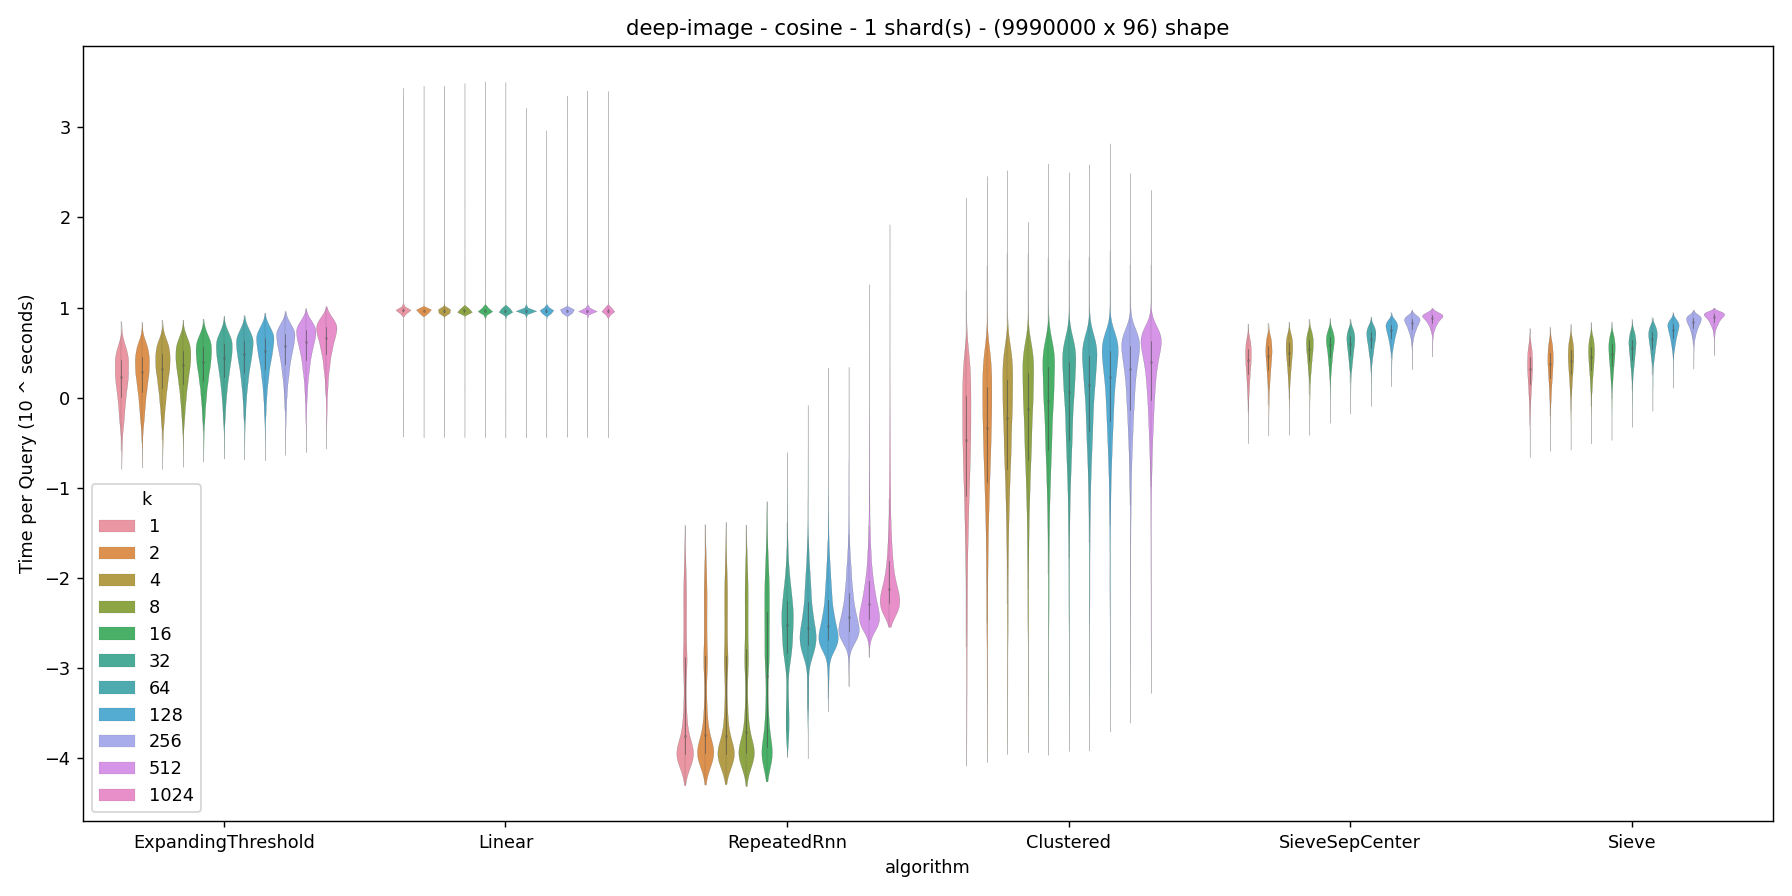
\includegraphics[width=3.4in]{images/result_plots/deep-image_1.png}
    \caption{Performance of CAKES algorithms on deep-image dataset.}
    \label{fig:methods:deep-image}
\end{figure}

Figure [ADD FIGURE NUMBER] is a violin plot which shows the performance of our algorithms
on [ADD DATASET] under [ADD DISTANCE FUNCTION] distance, using [ADD NUMBER OF SHARDS] shards.
As indicated in the title, the dataset has cardinality [ADD cardinality] and dimensionality [ADD DIMENSIONALITY].
On the horizontal axis, we have each of the $k$-NN algorithms described in Section 2.4, as well as  
an additional "algorithm" which we call "Oracle $\rho$-NN" [REPLACE WITH ACTUAL NAME].  With "Oracle $\rho$-NN", we perform $\rho$-NN search using the 
distance to the $k$-th nearest neighbor as the radius. Of course, as it is impossible to
to know the distance to the $k$-th nearest neighbor \emph{a priori}, this algorithm 
is useful only for benchmarking purposes.

The vertical axis for Figure [ADD FIGURE NUMBER] is the time query in seconds on a logarithmic scale. 
As shown in the key, different colors represent different values of $k$. 
The plot shows the distribution of query times for each algorithm for each value of $k$. 
Because of the logarithmic scale of the vertical axis, it is unsurprising that we 
see longer lower tails than upper tails for many of these algorithms. 


https://github.com/URI-ABD/clam

For each pair $(X, f)$ and a small selection of depths, measure:
\begin{enumerate}[1.]
    \item linear search vs accelerated search:
    \begin{enumerate}[i.]
        \item runtime performance,
        \item speedup factor, and
        \item number of distance comparisons.
    \end{enumerate}
\end{enumerate}

\begin{table*}[!t]
    % \renewcommand{\arraystretch}{1.15}
    \caption{Runtime performance (queries per second) of CAKES vs. other methods, $k=10$}
    \label{table:results:ann-10}
    \vskip 0.15in
    \begin{center}
    \begin{small}
    \begin{sc}
    \begin{tabular}{|l|p{1cm}|p{1cm}|p{1cm}|p{1cm}|p{1cm}|p{1cm}|p{1cm}|p{1cm}|}
    \textbf{Dataset}  & \multicolumn{2}{|c|}{\textbf{faiss-ivf}} & \multicolumn{2}{|c|}{\textbf{bruteforce-blas}} & \multicolumn{2}{|c|}{\textbf{hnsw(faiss)}} & \multicolumn{2}{|c|}{\textbf{CAKES}} \\
    \cline{2-9}
    &                    Recall & QPS                           & Recall & QPS                           & Recall & QPS                                           & Recall & QPS \\
    \hline
    fashion-mnist      & 1.000 & 188.03                           & 1.000 & 52.91                                  & 1.000* & 339.74                                                    & 1.000 & 16,220 \\
    \hline
    gist                   & 1.000 & 3.55                           & 1.000 & 2.63                                     & 0.953 & 149.58                                                   & 1.000 & 10,600 \\
    \hline
    glove-25              & 1.000 & 78.78                          & 1.000 & 33.52                              & 1.000 & 552.67                                                  & -- & 19,520 \\
    \hline
    glove-100             & 1.000 & 21.16                          & 1.000 & 16.52                                & 0.998 & 155.90                                                  & -- & 6,935 \\
    \hline
    sift                  & 1.000 &  24.52                          & 1.000 & 16.40                               & 1.000 & 275.07                                                    & 1.000 & 31,800 \\
    \hline
    \end{tabular}
    \end{sc}
    \end{small}
    \end{center}
    \vskip -0.1in
    \end{table*}


\begin{table*}[!t]
    % \renewcommand{\arraystretch}{1.15}
    \caption{Runtime performance (queries per second) of CAKES vs. other methods, $k=100$. Other methods did not report results for glove-25.}
    \label{table:results:ann-100}
    \vskip 0.15in
    \begin{center}
    \begin{small}
    \begin{sc}
    \begin{tabular}{|l|p{1cm}|p{1cm}|p{1cm}|p{1cm}|p{1cm}|p{1cm}|p{1cm}|p{1cm}|}
    \textbf{Dataset}  & \multicolumn{2}{|c|}{\textbf{faiss-ivf}} & \multicolumn{2}{|c|}{\textbf{bruteforce-blas}} & \multicolumn{2}{|c|}{\textbf{hnsw(faiss)}} & \multicolumn{2}{|c|}{\textbf{CAKES}} \\
    &                    Recall & QPS                           & Recall & QPS                           & Recall & QPS                                           & Recall & QPS \\
    \hline
    fashion-mnist         & 1.000 & 111.47                           & 1.000* & 16.02                                  & 1.000* & 277.80                                                    & 1.000 & 1,549 \\ 
    \hline
    gist                   & 1.000 & 2.70                           & 1.000* & 0.80                                 & 0.995 & 59.71                                                    & 1.000 & 753.9 \\
    \hline
    glove-25              & -- & --                                & -- & --                                & -- & --                                                    & -- & 1,471 \\
    \hline
    glove-100             & 1.000* &  19.04                          & 1.000* & 7.52                                 & 0.987 & 92.58                                                    & -- & 396.0 \\
    \hline
    sift                  & 1.000 &  23.50                          & 1.000 & 6.51                                  & 1.000* & 179.14                                                    & 1.000 & 2,852 \\                                                 
    \hline
    \end{tabular}
    \end{sc}
    \end{small}
    \end{center}
    \vskip -0.1in
    \end{table*}


    % \hline
    % deep-image             & 0.00 & 0.00                           & 0.00 & 0.00                                 & 0.00 & 0.00                                                     & 1.00 & 42 \\
    % \hline
    % mnist                   & 0.00 & 0.00                          & 0.00 & 0.00                                 & 0.00 & 0.00                                                    & 1.00 & 42 \\
    % \hline
    % glove-50               & 0.00 & 0.00                           & 0.00 & 0.00                              & 0.00 & 0.00                                                    & 1.00 & 42 \\
    % \hline
    % lastfm                 & 0.00 & 0.00                           & 0.00 & 0.00                               & 0.00 & 0.00   